\documentclass[11pt,a4paper]{article}
\usepackage[utf8]{inputenc}
\usepackage[margin=2.5cm]{geometry}
\usepackage{graphicx}
\usepackage{float}
\usepackage{xcolor}
\usepackage{listings}
\usepackage{hyperref}
\usepackage{graphicx}

\graphicspath{ {./images/} }

\title{Behind the Scenes}
\author{Carlo Ramponi}
\date{22 April 2022}

\definecolor{codegreen}{rgb}{0,0.6,0}
\definecolor{codegray}{rgb}{0.5,0.5,0.5}
\definecolor{codepurple}{rgb}{0.58,0,0.82}
\definecolor{backcolour}{rgb}{0.95,0.95,0.92}

\lstdefinestyle{mystyle}{
    backgroundcolor=\color{backcolour},   
    commentstyle=\color{codegreen},
    keywordstyle=\color{magenta},
    numberstyle=\tiny\color{codegray},
    stringstyle=\color{codepurple},
    basicstyle=\ttfamily\footnotesize,
    breakatwhitespace=false,         
    breaklines=true,                 
    captionpos=b,                    
    keepspaces=true,                 
    numbers=left,                    
    numbersep=5pt,                  
    showspaces=false,                
    showstringspaces=false,
    showtabs=false,                  
    tabsize=2
}

\lstset{style=mystyle}

\begin{document}
\begin{titlepage}

\centering
    \vfill
    \vskip3cm
    \Large Department of Information Engineering and Computer Science
    \vskip0.5cm
    \Large (DISI)
    \vskip2cm
    
\includegraphics[width=8cm]{images/logo_unitn.png}
    \vskip2cm
    \textbf{\Large Network Security - A.Y. 2021/2022}
    \vskip2cm
    \textbf{\LARGE DNS}
    \vskip0.2cm
    \textbf{\LARGE Cache poisoning and Kaminsky attack}
    \vskip4cm
    \Large Carlo Ramponi, Luca De Menego, Matteo Zanotto
    \vfill

\end{titlepage}

\clearpage

\tableofcontents

\clearpage

\section{DNS specification}

\subsection{What is the DNS}

\subsection{Typical messages flow}

\subsection{DNS messages format}

\subsection{Resources representation}

\section{DNS implementation: Bind}

\subsection{Bind configuration}

\subsection{Zone files}

\section{Laboratory introduction}

\subsection{Katharà}

\subsection{Laboratory network topology}
\subsection{DNSSEC}
\begin{figure}[h]
  \centering
  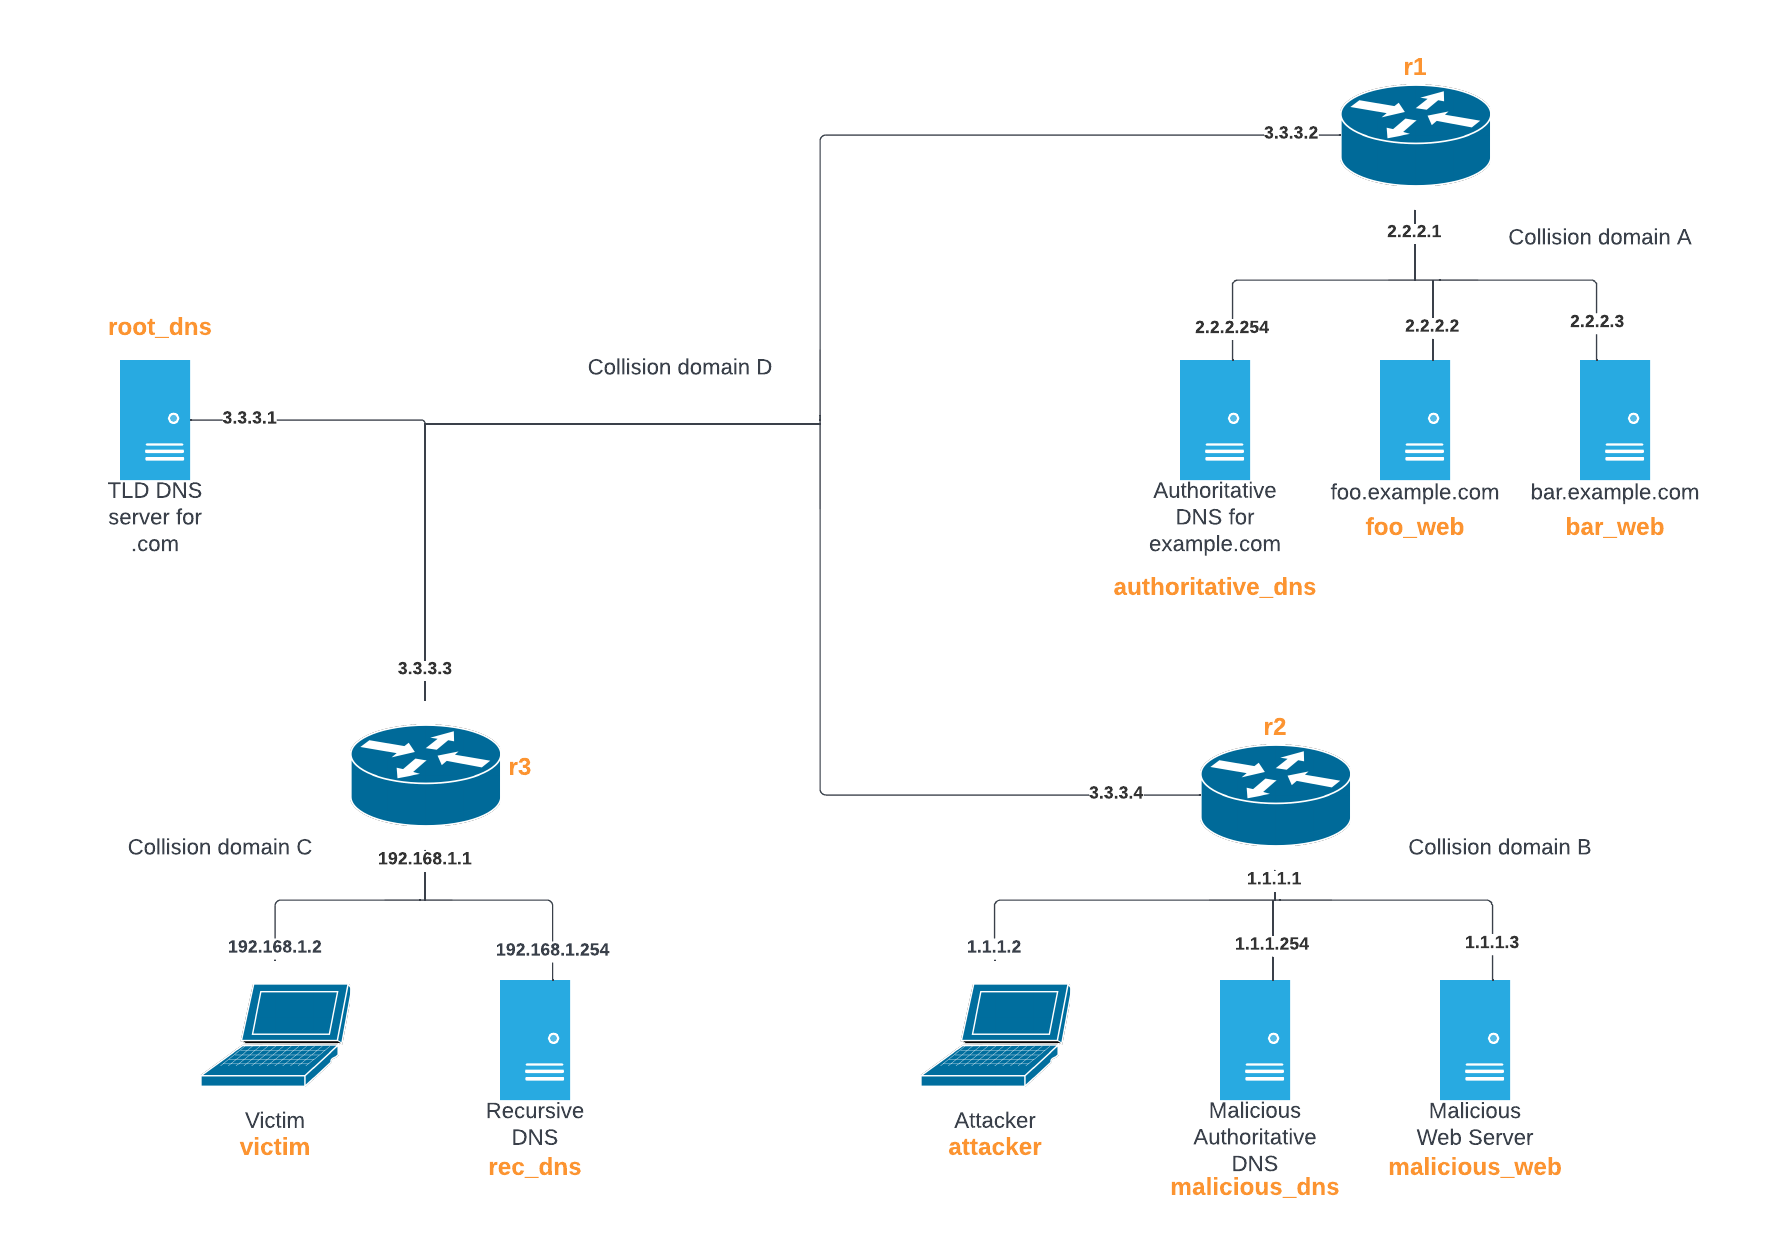
\includegraphics[scale=0.56]{network-topology.png}
  \caption{Laboratory network topology}
\end{figure}

\section{Final considerations}

\subsection{Performing the attack nowadays}

\subsection{DNSSEC}

\end{document}